\chapter{Transport layer protocols}
\label{chap:transport}

\section{\acl{UDP}}
\label{sec:udp}

\paragraph{header}
A \acs{UDP} datagram consists of a datagram header followed by a data section (the payload data for the application).
The \acs{UDP} datagram header consists of four fields, each of which is two bytes (16~bits).

\begin{figure}
\begin{sidecaption}{The \acs{UDP} header}[fig:transport-udp-header]
\begin{bytefield}{32}
\bitheader{0,15,16,31} \\
\bitbox{16}{source port}
\bitbox{16}{destination port} \\
\bitbox{16}{length}
\bitbox{16}{checksum} \\
\end{bytefield}
\end{sidecaption}
\end{figure}

The length field specifies the length in bytes of the \acs{UDP} header and \acs{UDP} data.
The minimum length is eight bytes, the length of the header.
   
\paragraph{port numbers}
   \index{port number}
In computer networking, a port is a communication endpoint.
At the software level, within an operating system, a port is a logical construct that identifies a specific process or a type of network service.
A port is identified for each transport protocol and address combination by a 16-bit unsigned number, known as the \emph{port number}.

A port number is always associated with an \acs{IP} address of a host and the type of transport protocol used for communication.
It completes the destination or the originating network address of a message.
Specific port numbers are reserved to identify specific services so that an arriving packet can be easily forwarded to a running application.
For this purpose, port numbers lower than 1024 identify the historically most commonly used services and are called the \emph{well-known port numbers}.
Higher-numbered ports are available for general use by applications and are known as \emph{ephemeral ports}.
   \index{port number!well-known}
   \index{port number!ephemeral}
 
\Vref{tab:port-numbers} lists a few well-known port numbers while \vref{tab:ephemeral-ports} lists the range of ephemeral port numbers used by some operating systems.
Note that, although both \acs{UDP} and \acs{TCP} use port numbers and they both look identical, they are both distinct.
One application can use \acs{UDP} port~500 while another application can use \acs{TCP} port~500.
Since the protocol is different, the ports are different as well and one application will not receive network packets destined for the other application.

\begin{margintable}
\centering
\begin{tabular}{ll}
\acs{TCP}/22 & \acs{SSH}           \\
\acs{TCP}/25 & \acs{SMTP}          \\
\acs{UDP}/53 & \acs{DNS}           \\
\acs{UDP}/67 & \acs{DHCP} (server) \\
\acs{UDP}/68 & \acs{DHCP} (client) \\
\acs{TCP}/80 & \acs{HTTP}          \\
\acs{TCP}/110 & \acs{POP3} \\
\acs{UDP}/123 & \acs{NTP} \\
\acs{TCP}/143 & \acs{IMAP} \\
\acs{TCP}/443 & \acs{HTTPS} \\
\acs{TCP}/445 & \acs{SMB} file shares \\
\end{tabular}
\caption{A few well-known ports}
\label{tab:port-numbers}
\end{margintable}

\begin{margintable}
\centering
\begin{tabular}{lr@{--}l}
Linux        & \numprint{32768} & \numprint{60999} \\
FreeBSD      & \numprint{49152} & \numprint{65535} \\
Windows XP   & \numprint{1025} & \numprint{5000} \\
Windows 7    & \numprint{49152} & \numprint{65535} \\
\end{tabular}
\caption{Port ranges used by operating systems as ephemeral ports}
\label{tab:ephemeral-ports}
\end{margintable}
   
In practice when a company requested a port number for use by its application, it was given both the \acs{UDP} and the \acs{TCP} port number.
This turned out to be really convenient as \acs{DNS} started out using only \acs{UDP} but now also uses \acs{TCP}.\iacs{DNS}
As it was given both \acs{UDP}/53 and \acs{TCP}/53, it can use the same port number for both protocols.


\paragraph{checksum}
   \index{checksum}
A checksum is a small-sized block of data derived from another block of digital data for the purpose of detecting errors that may have been introduced during its transmission or storage.
By themselves, checksums are often used to verify data integrity but are not relied upon to verify data authenticity.

\paragraph{`unreliable'}
The \ac{UDP} does not keep track of which packets have been sent or received correctly.
It just sends data and forgets about it.
Should the application require reliability, it itself is responsible for this function.
This lack of reliability makes \ac{UDP} a very fast protocol.









\section{\acl{TCP}}
\label{sec:tcp}


\paragraph{port numbers and checksum}
See \cref{sec:udp}.

\paragraph{`reliable'}
The \ac{TCP} makes sure all data that is sent, is also received correctly by the destination.
It uses a combination of \emph{sequence numbers} and \emph{acknowledgements} to achieve this reliability.

\paragraph{three-way handshake}
   \index{three-way handshake}
Before a client attempts to connect with a server, the server must first bind to and listen at a port to open it up for connections: this is called a passive open.
Once the passive open is established, a client may establish a connection by initiating an active open using the three-way handshake.%
   \index{TCP@\acs{TCP}!passive open}

\begin{marginfigure}
\fxwarning[layout=inline]{Create or steal this image.}
\caption{The three-way handshake}
\label{fig:transport-three-way-handshake}
\end{marginfigure}

\begin{description}
\item[\SC{SYN}]
The active open is performed by the client sending a \SC{SYN} to the server.
The client sets the segment's sequence number to a random value $A$.%
    \footnote{%
        The Wireshark\index{Wireshark} capture in \cref{tab:tcp-handshake} gives a sequence number of zero.
        This is because of WireShark option called `Relative sequence numbers' which lets the numbers start from zero to make them more easy to read by humans.
        It does this by subtracting the initial value $A$ in the \SC{SYN} packet from the value in all subsequent packets sent by the client and subtracting the initial value $B$ from all subsequent packets sent by the server.
        }
\item[\SC{SYN+ACK}]
In response, the server replies with a \SC{SYN+ACK}.
The acknowledgement number is set to one more than the received sequence number i.e. $A+1$, and the sequence number that the server chooses for the packet is another random number, $B$.
\item[\SC{ACK}]
Finally, the client sends an \SC{ACK} back to the server.
The sequence number is set to the received acknowledgement value i.e. $A+1$, and the acknowledgement number is set to one more than the received sequence number i.e. $B+1$.
\end{description}
Steps 1 and 2 establish and acknowledge the sequence number for one direction.
Steps~2 and~3 establish and acknowledge the sequence number for the reverse direction.
Following the completion of these steps, both the client and server have received acknowledgements and a full-duplex (\acs{FDX}) communication is established.

\begin{table}
\centering
\begin{tabular}{rlll}
{\#} & {source} & {destination} & {info} \\
\midrule
1 & 10.0.0.1 & 203.0.113.80 & 53501 $\rightarrow$ 443 [\SC{SYN}] seq=0 win=64240 \dots\\
2 & 203.0.113.80 & 10.0.0.1 & 443 $\rightarrow$ 53501 [\SC{SYN}, \SC{ACK}] seq=0 ack=1 \dots\\
3 & 10.0.0.1 & 203.0.113.80 & 53501 $\rightarrow$ 443 [\SC{ACK}] seq=1 ack=1 \ldots\\
\end{tabular}
\caption{A few fields that Wireshark shows about a three-way handshake}
\label{tab:tcp-handshake}
\end{table}

\paragraph{acknowledgements}
\ac{TCP} uses sequence numbers to identify each byte of data.
The sequence number identifies the order of the bytes sent from each computer so that the data can be reconstructed in order, regardless of any out-of-order delivery that may occur.
The sequence number of the first byte is chosen by the transmitter for the first packet, which is flagged \SC{SYN}.
This number can be arbitrary, and should, in fact, be unpredictable to defend against \ac{TCP} sequence prediction attacks.

When the receiver sends an acknowledgement (\SC{ACK}) the sequence number indicates till which byte the data has been received.
Acknowledgements do not imply that the data has been delivered to the application, they merely signify that it is now the receiver's responsibility to deliver the data.

Reliability is achieved by the sender detecting lost data and retransmitting it.
\ac{TCP} uses two primary techniques to identify loss: \acf{RTO} and duplicate cumulative acknowledgements.%
   \index{retransmission timeout}

\fxwarning{Explain RTO briefly}

\fxwarning{You cannot leave the audience hanging like this. Either explain both or tell them where/when it will be explained. I cannot quickly find the explanation myself in this text.}

\paragraph{flow control}
   \index{TCP@\acs{TCP}!flow control}
   \index{TCP@\acs{TCP}!sliding window}
   \index{TCP@\acs{TCP}!receive window}
\acs{TCP} uses a \emph{sliding window} flow control protocol.
In each \acs{TCP} segment, the receiver specifies in the \emph{receive window} field the amount of additionally received data (in bytes) that it is willing to buffer for the connection.
The sending host can send only up to that amount of data before it must wait for an acknowledgement and receive window update from the receiving host.


\begin{figure}
\centering
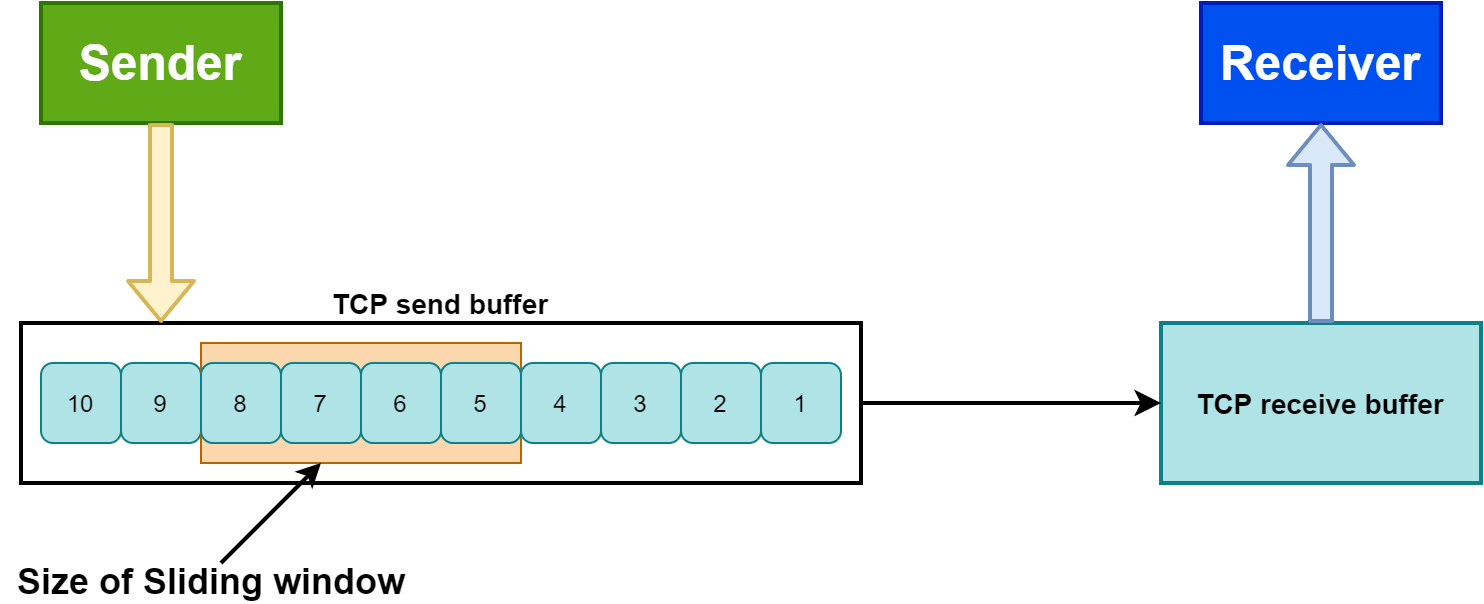
\includegraphics[width=.7\textwidth]{images/transport/flow-control.png}
\caption{\acs{TCP} flow control using a sliding window}
\label{fig:flow-control}
\end{figure}

\paragraph{congestion control}
   \index{TCP@\acs{TCP}!congestion control}
The final main aspect of \acs{TCP} is congestion control.
\acs{TCP} uses a number of mechanisms to achieve high performance and avoid congestion collapse, where network performance can fall by several orders of magnitude.
These mechanisms control the rate of data entering the network, keeping the data flow below a rate that would trigger collapse.
They also yield an approximately min--max fair allocation between flows.

Acknowledgements for data sent, or lack of acknowledgements, are used by senders to infer network conditions between the \acs{TCP} sender and receiver.
Coupled with timers, \acs{TCP} senders and receivers can alter the behavior of the flow of data.
This is more generally referred to as \emph{congestion control} and/or \emph{network congestion avoidance}.

Modern implementations of \acs{TCP} contain four intertwined algorithms: \emph{slow start}, congestion avoidance, \emph{fast retransmit}, and \emph{fast recovery} (\rfc{5681}).


\extrap{slow start}
   \index{TCP@\acs{TCP}!slow start}
% https://www.stackpath.com/edge-academy/what-is-tcp-slow-start/
\acs{TCP} slow start is an algorithm which balances the speed of a network connection.
Slow start gradually increases the amount of data transmitted until it finds the network's maximum carrying capacity.

\extrap{congestion avoidance}
   \index{TCP@\acs{TCP}!congestion avoidance}
If a loss event occurs, \acs{TCP} assumes that it is due to network congestion and takes steps to reduce the offered load on the network.
These measurements depend on the exact \acs{TCP} congestion avoidance algorithm used.

\extrap{fast retransmit}
   \index{TCP@\acs{TCP}!fast retransmit}
Fast retransmit is an enhancement to \acs{TCP} that reduces the time a sender waits before retransmitting a lost segment.
A \acs{TCP} sender normally uses a simple timer to recognize lost segments.
If an acknowledgement is not received for a particular segment within a specified time (a function of the estimated round-trip delay time), the sender will assume the segment was lost in the network, and will retransmit the segment.

Duplicate acknowledgement is the basis for the fast retransmit mechanism.
   \index{TCP@\acs{TCP}!duplicate acknowledgement}
After receiving a packet an acknowledgement is sent for the last in-order byte of data received.
For an in-order packet, this is effectively the last packet's sequence number plus the current packet's payload length.
If the next packet in the sequence is lost but a third packet in the sequence is received, then the receiver can only acknowledge the last in-order byte of data, which is the same value as was acknowledged for the first packet.
The second packet is lost and the third packet is not in order, so the last in-order byte of data remains the same as before.
Thus a duplicate acknowledgement occurs.
The sender continues to send packets, and a fourth and fifth packet are received by the receiver.
Again, the second packet is missing from the sequence, so the last in-order byte has not changed.
Duplicate acknowledgements are sent for both of these packets.

When a sender receives three duplicate acknowledgements, it can be reasonably confident that the segment carrying the data that followed the last in-order byte specified in the acknowledgment was lost. 
A sender with fast retransmit will then retransmit this packet immediately without waiting for its timeout.
On receipt of the retransmitted segment, the receiver can acknowledge the last in-order byte of data received.
In the above example, this would acknowledge to the end of the payload of the fifth packet.
There is no need to acknowledge intermediate packets, since \acs{TCP} uses cumulative acknowledgements by default.

\extrap{fast recovery}
   \index{TCP@\acs{TCP}!fast recovery}
\fxwarning{Write something about \acs{TCP} fast recovery.}



\section{Load balancing}
\fxwarning{Write something about load balancing.}
Load balancing is the process of distributing a set of tasks over a set of resources (computing units), with the aim of making their overall processing more efficient.


\section{Review questions}
\label{sec:transport-review-qu}



\section{Guided exercises}
\label{sec:transport-guided-ex}



\section{Practice questions}
\label{sec:transport-practice-qu}




\section{Further reading}
Both \textcite{stevens,comer} are good resources to learn more about how the \acf{TCP} operates.
Additionally you can take a look at the actual network packets as they are being sent and received on the network.
This requires a software tool like Wireshark to capture and display the packets.%
   \index{Wireshark}
To learn how this program works, Chris Greer, a leading expert on packet analysis, recommends \textcite{chappell17,sanders,bock}.
I own a different book by \citeauthor{chappell17} but I am unfamiliar with these three recommended books.
